
\documentclass{l4proj}

%
% put any packages here
%

\begin{document}
\title{Augmented Reality Android Gym App}
\author{David Benicek 2073063b}
\date{\today}
\maketitle

\begin{abstract}
Something will go here.
\end{abstract}

\educationalconsent
%
%NOTE: if you include the educationalconsent (above) and your project is graded an A then
%      it may be entered in the CS Hall of Fame
%
\tableofcontents
%==============================================================================

\chapter{Introduction}
\pagenumbering{arabic}


\begin{verbatim}

            > pdflatex example0
            > bibtex example0
            > pdflatex example0
            > pdflatex example0

\end{verbatim}


\section{Motivation}
The quick brown fox jumped over the lazy dog.
The quick brown fox jumped over the lazy dog.
The quick brown fox jumped over the lazy dog.
The quick brown fox jumped over the lazy dog.
The quick brown fox jumped over the lazy dog.
The quick brown fox jumped over the lazy dog.
The quick brown fox jumped over the lazy dog.
The quick brown fox jumped over the lazy dog.

\section{Background}
The quick brown fox jumped over the lazy dog.
The quick brown fox jumped over the lazy dog.
The quick brown fox jumped over the lazy dog.
The quick brown fox jumped over the lazy dog.

The quick brown fox jumped over the lazy dog.
The quick brown fox jumped over the lazy dog.
The quick brown fox jumped over the lazy dog.
The quick brown fox jumped over the lazy dog.

\section{Aim}
The quick brown fox jumped over the lazy dog.
The quick brown fox jumped over the lazy dog.
The quick brown fox jumped over the lazy dog.
The quick brown fox jumped over the lazy dog.
The quick brown fox jumped over the lazy dog.
The quick brown fox jumped over the lazy dog.
The quick brown fox jumped over the lazy dog.
The quick brown fox jumped over the lazy dog.

\section{Outline}
The quick brown fox jumped over the lazy dog.
The quick brown fox jumped over the lazy dog.
The quick brown fox jumped over the lazy dog.
The quick brown fox jumped over the lazy dog.
The quick brown fox jumped over Uroborus (Figure \ref{uroborus}).
The quick brown fox jumped over the lazy dog.

The quick brown fox jumped over the lazy dog.
The quick brown fox jumped over the lazy dog.
The quick brown fox jumped over the lazy dog.
The quick brown fox jumped over the lazy dog.
The quick brown fox jumped over the lazy dog.
The quick brown fox jumped over the lazy dog.
The quick brown fox jumped over the lazy dog.
The quick brown fox jumped over the lazy dog.
The quick brown fox jumped over the lazy dog.
The quick brown fox jumped over the lazy dog.
The quick brown fox jumped over the lazy dog.

\chapter{Requirement}
The quick brown fox jumped over the lazy dog.
The quick brown fox jumped over the lazy dog.
The quick brown fox jumped over the lazy dog.
The quick brown fox jumped over the lazy dog.

\section{Requirements gathering}
The quick brown fox jumped over the lazy dog.
The quick brown fox jumped over the lazy dog.
The quick brown fox jumped over the lazy dog.
The quick brown fox jumped over the lazy dog.
\subsection{Questionnaire}
The quick brown fox jumped over the lazy dog.
The quick brown fox jumped over the lazy dog.
The quick brown fox jumped over the lazy dog.
The quick brown fox jumped over the lazy dog.
\subsection{Meeting with GUSA}
The quick brown fox jumped over the lazy dog.
The quick brown fox jumped over the lazy dog.
The quick brown fox jumped over the lazy dog.
The quick brown fox jumped over the lazy dog.

\chapter{Design}
\section{User Experience}
The quick brown fox jumped over the lazy dog.
The quick brown fox jumped over the lazy dog.
The quick brown fox jumped over the lazy dog.
The quick brown fox jumped over the lazy dog.
\section{User Interface}
The quick brown fox jumped over the lazy dog.
The quick brown fox jumped over the lazy dog.
The quick brown fox jumped over the lazy dog.
The quick brown fox jumped over the lazy dog.

\chapter{Implementation}
\chapter{Testing}

\chapter{Conclusion}

\chapter{Evaluation}

%\vspace{-7mm}
\begin{figure}
\centering
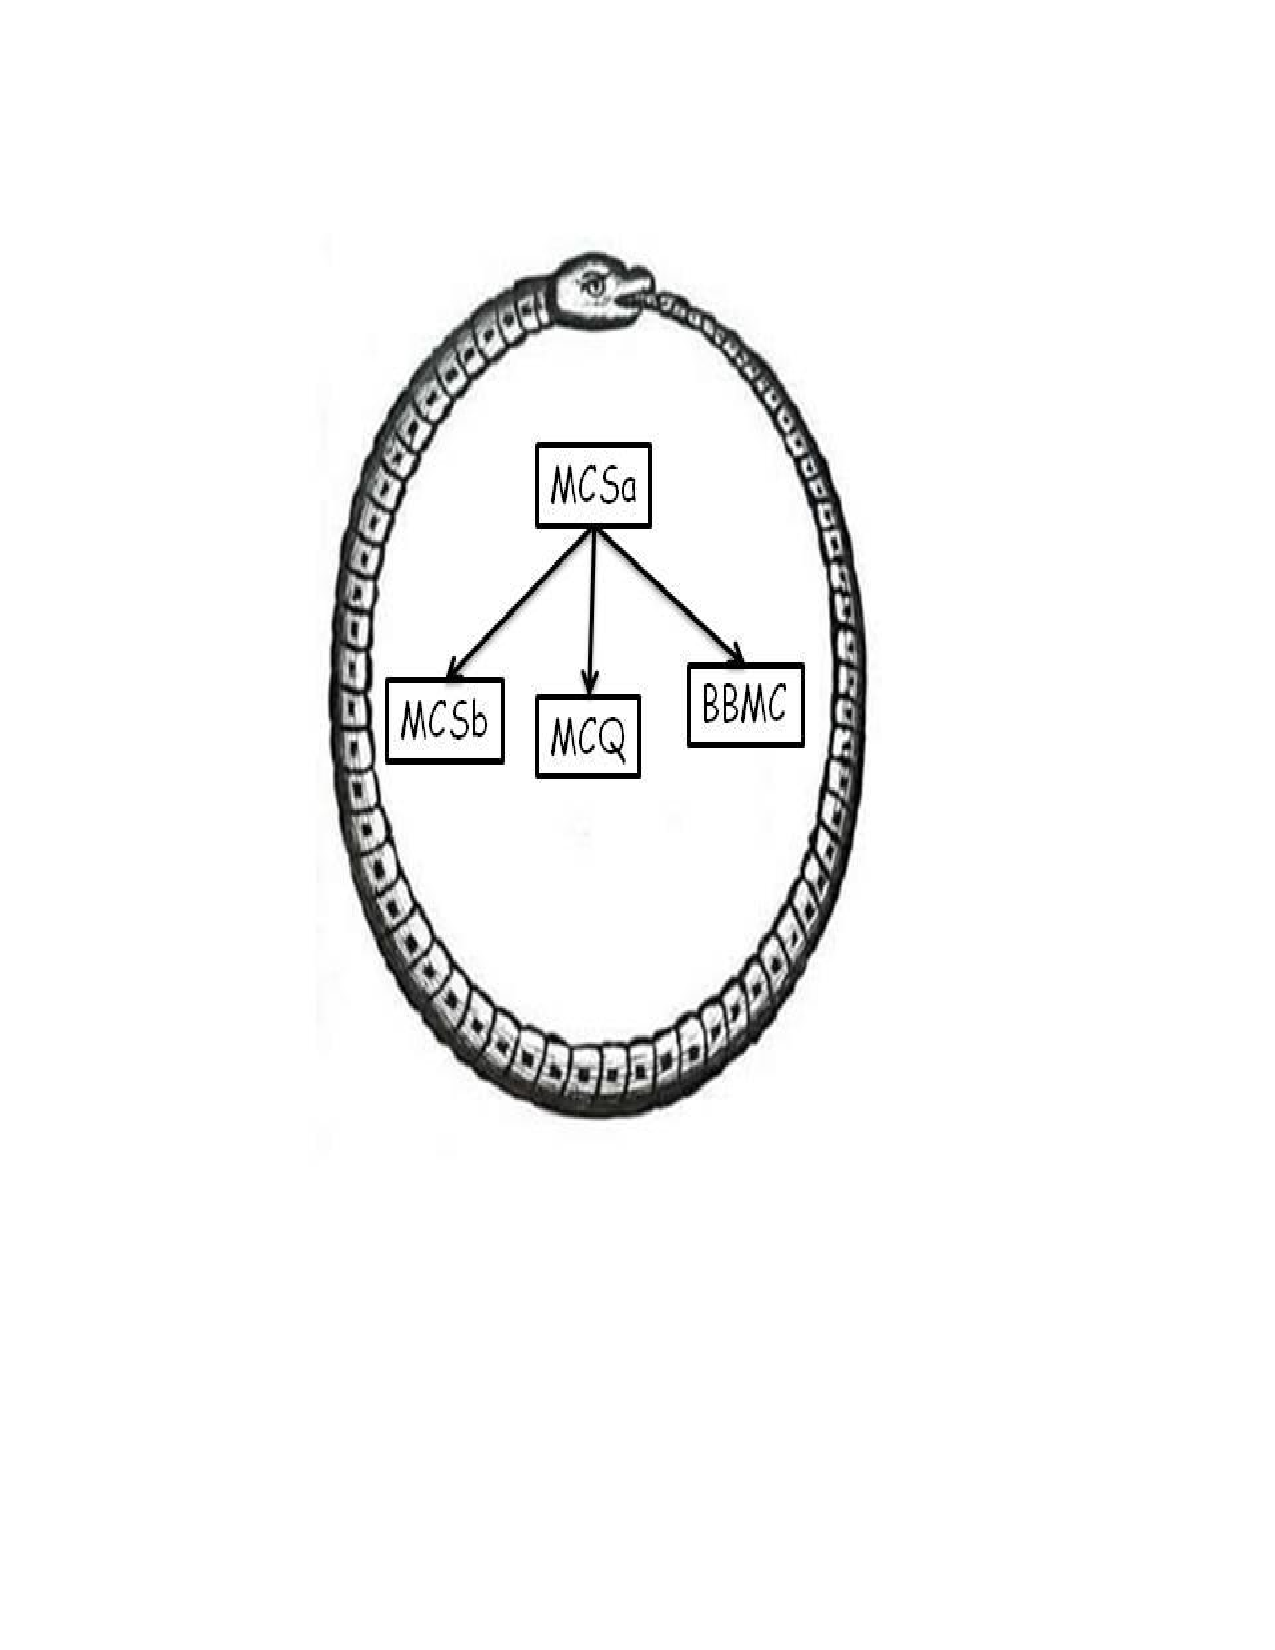
\includegraphics[height=9.2cm,width=13.2cm]{uroboros.pdf}
\vspace{-30mm}
\caption{An alternative hierarchy of the algorithms.}
\label{uroborus}
\end{figure}



%%%%%%%%%%%%%%%%
%              %
%  APPENDICES  %
%              %
%%%%%%%%%%%%%%%%
\begin{appendices}

\chapter{Running the Programs}
An example of running from the command line is as follows:
\begin{verbatim}
      > java MaxClique BBMC1 brock200_1.clq 14400
\end{verbatim}
This will apply $BBMC$ with $style = 1$ to the first brock200 DIMACS instance allowing 14400 seconds of cpu time.

\chapter{Generating Random Graphs}
\label{sec:randomGraph}
We generate Erd\'{o}s-R\"{e}nyi random graphs $G(n,p)$ where $n$ is the number of vertices and
each edge is included in the graph with probability $p$ independent from every other edge. It produces
a random graph in DIMACS format with vertices numbered 1 to $n$ inclusive. It can be run from the command line as follows to produce 
a clq file
\begin{verbatim}
      > java RandomGraph 100 0.9 > 100-90-00.clq
\end{verbatim}
\end{appendices}

%%%%%%%%%%%%%%%%%%%%
%   BIBLIOGRAPHY   %
%%%%%%%%%%%%%%%%%%%%

\bibliographystyle{plain}
\bibliography{bib}

\end{document}
